\documentclass[a4paper,12pt]{article} 
\usepackage[utf8x]{inputenc}
\usepackage[french]{babel}
\usepackage{mathtools}
\usepackage{amsmath}
\usepackage{amsfonts}
\usepackage{amssymb}
\usepackage{graphicx}		 			% Inclusion des figures 
\usepackage{textcomp}
\usepackage[nointegrals]{wasysym}			% Collection de symboles mathématiques
\usepackage{multicol}					% Pour utiliser \hfill
\usepackage{ifthen}
\usepackage{tabularx}	 				% Gestion avancée des tableaux
%\usepackage{cleveref}

\usepackage{enumitem}
\usepackage{wrapfig}
%\usepackage[squaren]{SIunits}
%\usepackage[T1]{fontenc}				% Indispendable, présent dans tous les codes exemples

\usepackage[linkcolor=DarkRed,colorlinks=true, citecolor= DarkGreen, urlcolor=MidnightBlue]{hyperref} 	% Hyper ref

\usepackage[justification=centering]{caption}
\usepackage{sistyle} 
\usepackage{numprint}
\usepackage{wrapfig}
\usepackage{cite}	
\usepackage{url} 					% Pour citer les sites internet dans la
%\usepackage{cleveref}
\usepackage{setspace}

\usepackage[svgnames]{xcolor}			%https://www.latextemplates.com/svgnames-colors

%%% Couleurs %%%
\xdefinecolor{brick}{named}{DarkRed}
\xdefinecolor{navy}{named}{Navy}
\xdefinecolor{midblue}{named}{MidnightBlue}
\xdefinecolor{dsb}{named}{DarkSlateGray}
\xdefinecolor{dgreen}{named}{DarkGreen}

\newcommand{\bepar}[1]{
	\left( #1 \right)  
}

\newcommand{\becro}[1]{
	\left[ #1 \right]  
}

%%% Élément pour citer des codes %%%
\usepackage{listings}
\lstset{
		language=bash,
		basicstyle=\ttfamily\bfseries\small, %
		identifierstyle=\bfseries\color{black}, %
		keywordstyle=\color{blue}, %
		stringstyle=\color{FireBrick}, %
		commentstyle=\it\color{black!80!red!85!}, %
		columns=flexible, %
		tabsize=8, %
		extendedchars=true, %
		showspaces=false, %
		showstringspaces=false, % %
		numberstyle=\small, %
		breaklines=true, %
		breakautoindent=true, %
		captionpos=b,
		escapeinside={<*}{*>}
		}


\title{How to use git}%%%%%%%%%%%%%%%%%%%%
\date{}
\usepackage{multicol}
\usepackage{etoolbox}

\patchcmd{\thebibliography}{\section*{\refname}}
    {\begin{multicols}{2}[\section*{\refname}]}{}{}
\patchcmd{\endthebibliography}{\endlist}{\endlist\end{multicols}}{}{}

\usepackage{geometry}
\geometry{hmargin=1.5cm, vmargin=2cm}

%%%%%%%%%%%%%%%%%%%%

%%% 	Raccourcis 	%%%
\newcommand{\keps}{$k-\varepsilon$}
\newcommand\bk{\color{black}}
\newcommand\brick{\color{brick}}
\newcommand\navy{\color{navy}}
\newcommand\midblue{\color{midblue}}
\newcommand\dsb{\color{dsb}}
\newcommand{\dgreen}{\color{dgreen}}

%%%%%%%% Cigles
\newcommand{\rap}{par rapport }
\newcommand{\cad}{c'est-à-dire}

%%%%%%%% Autres

%%%%%%%%%%%%%%%%%%%
% Syntax: \colorboxed[<color model>]{<color specification>}{<math formula>}
\newcommand*{\colorboxed}{}
\def\colorboxed#1#{%
  \colorboxedAux{#1}%
}
\newcommand*{\colorboxedAux}[3]{%
  % #1: optional argument for color model
  % #2: color specification
  % #3: formula
  \begingroup
    \colorlet{cb@saved}{.}%
    \color#1{#2}%
    \boxed{%
      \color{cb@saved}%
      #3%
    }%
  \endgroup
}
\renewcommand{\sectionmark}[1]{\markright{#1}}
\usepackage{fancyhdr}
\pagestyle{fancy}
\lhead{\textbf{Nathaniel} \brick \textbf{\textsc{Saura}}}
\rhead{\markright}
\cfoot{\thepage}
\renewcommand{\headrulewidth}{0.4pt}

\numberwithin{equation}{section} %%%% To count the equation like Section.Number

% Pour désactiver l'indentation automatique :
\setlength\parindent{0pt}

%%%%%%%%%%%%%%%%%%%

\begin{document}
\maketitle

\begin{center}
Provient de \\ \url{https://git-scm.com/book/fr/v1/Les-bases-de-Git-Enregistrer-des-modifications-dans-le-d%C3%A9p%C3%B4t} 
\end{center}

\vspace{4mm}
\flushleft
Git thinks of its data more like a series of snapshots of a miniature filesystem.\\
Each commit is actually a picture of the file at the moment and stores a reference to that snapshots.\\
If the file hasn't changed, Git doesn't store the file again. \textbf{Data are then a stream of snapshots}\\

Entire project sotry is saved locally $\Rightarrow$ Most operation seems almost instanteneous. It can so browse the history of the file directly from the local database. So it is for the comparison of two different version: Git performs local difference calculations.\\[3mm]

Three states for files : commited (validé), modified (modifié) and staged (index) :
	\begin{itemize}
		\item[--] Commited : data safely stored in the local database; \\
		\item[--] Modified : file has changed but has not been commited yet; \\
		\item[--] Staged   : modified file marked to be the next snapshot. \\[6mm]
	\end{itemize} 

Basic Git workflow :
	\begin{itemize}
		\item[--] Modify a file;\\
		\item[--] Selectively stage the changes you want to be part of the next commit, which adds only these wanted changes to the staging area. This «area» is actually a file that stores information about what it is expected to happend at the next commit;\\
		\item[--] Do a commit : takes the files as they are in the stage area and stores that snapshots permanently in the Git directory. \\[6mm]
	\end{itemize}


To install it is recommended to do 
\begin{lstlisting}
	<*\colorbox{gray!30!}{\textcolor{FireBrick}{sudo apt-get install git-all}}*> 
\end{lstlisting}
Then you can configure the git by specifying global items for example :
\begin{lstlisting}
	<*\colorbox{gray!30!}{\textcolor{FireBrick}{git config --global user.name "Nathaniel Saura"}}*>
	<*\colorbox{gray!30!}{\textcolor{FireBrick}{git config --global user.email "saura.nathaniel@gmail.com"}}*>
\end{lstlisting}
To see all the setting :
\begin{lstlisting}
	<*\colorbox{gray!30!}{\textcolor{FireBrick}{git config --list}}*>
\end{lstlisting}

We can ask help for each git command. For exemple :
\begin{lstlisting}
	<*\colorbox{gray!30!}{\textcolor{FireBrick}{git config -h}}*>
	<*\colorbox{gray!30!}{\textcolor{FireBrick}{git add -h}}*>
\end{lstlisting}

\pagebreak

\section*{Recording Changes to the Repository}
Each file in the WD (working directory) can be in one of two states : \textit{tracked} or \textit{untracked}

\begin{itemize}
	\item[--] Tracked files : files which were in the last snapshot, they can be unmodified, modified or stacked. \textbf{Git knows them}; \\
	\item[--] Untracked files : everything else, files that were not in the last snapshot nor in current staged area.\\[6mm]
\end{itemize}

\begin{figure}[!ht]
\centering
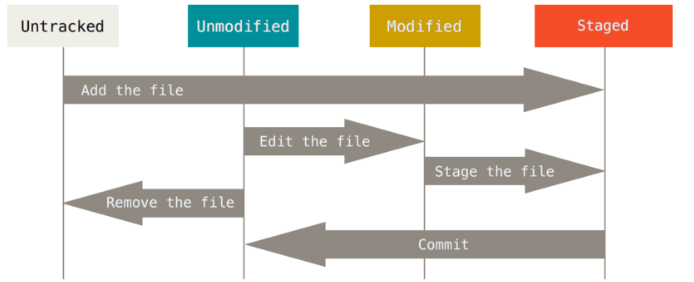
\includegraphics[scale=0.7]{./pic/file_states.png}
\end{figure}

\subsection*{Check the status :}
\begin{lstlisting}
	<*\colorbox{gray!30!}{\textcolor{FireBrick}{git status}}*>
\end{lstlisting}

If we add a new file README, and we check the status (before any commiting or adding)
\begin{lstlisting}
<*\textcolor{navy}{Untracked files:}*>
  (use "git add <file>..." to include in what will be committed)

	README

nothing added to commit but untracked files present (use "git add" to track)
\end{lstlisting}
It is necessary to specify that this file is wanted. \\[4mm]

\subsection*{Tracking new files :}
\begin{lstlisting}
	<*\colorbox{gray!30!}{\textcolor{FireBrick}{git add README}}*>
\end{lstlisting}
\begin{lstlisting}
Your branch is up-to-date with 'origin/master'.
<*\textcolor{navy}{Changes to be committed}*>:
(use "git reset HEAD <file>..." to unstage)
new file:
README
\end{lstlisting}
README is staged because under the \navy Changes to be committed \bk.\\ \textsc{git add} on a directory will add recursively every files in this directory. \\[4mm]

\pagebreak

\subsection*{Staging Modified Files}
When a tracked file is the modified this error message is displayed 
\begin{lstlisting}
<*\textcolor{navy}{Changes not staged for commit}*>:
  (use "git add <file>..." to update what will be committed)
  (use "git checkout -- <file>..." to discard changes in working directory)

	modified:   README
\end{lstlisting}

For now on we will use the command 
\begin{lstlisting}
	<*\colorbox{gray!30!}{\textcolor{FireBrick}{git status -s}}*>
\end{lstlisting}
The output is something like that for example
\begin{lstlisting}
$ git status -s
M README
MM Rakefile
A lib/git.rb
M lib/simplegit.rb
?? LICENSE.txt
\end{lstlisting}
The non obvious one is MM that means \textit{modified, staged and modified again}.

\subsection*{Ignoring files}
Generally files that are automatically created (logs, .o etc).\\
Have to modify \textit{.gitignore} :
\begin{lstlisting}
cat .gitignore
*.[oa] files that ends with .o or .a
*~	   files that ends with ~, generally temporary files
*.pyc  in practice
\end{lstlisting}

There are a lot of different options when building .gitignore here another more useful example :
\begin{lstlisting}
*.a # ignore all .a files

!lib.a # but do track lib.a, even though you're ignoring .a files above

/TODO # only ignore the TODO file in the current directory, not subdir/TODO

build/ # ignore all files in any directory named build

doc/*.txt # ignore doc/notes.txt, but not doc/server/arch.txt

doc/**/*.pdf # ignore all .pdf files in the doc/ directory and any of its subdirectories
\end{lstlisting}

\paragraph*{NOTE} : the shortcut *.[several ext] doesn't to work. One should write in row every exception. To delete gitignore-d files one can write :
\begin{lstlisting}
	<*\colorbox{gray!30!}{\textcolor{FireBrick}{git rm -r --cached .}}*>
	<*\colorbox{gray!30!}{\textcolor{FireBrick}{git add .}}*>
	<*\colorbox{gray!30!}{\textcolor{FireBrick}{git commit -m "mess about cancelation"}}*>
\end{lstlisting}

\pagebreak 

\subsection*{See the history}
\begin{lstlisting}
	<*\colorbox{gray!30!}{\textcolor{FireBrick}{git log --stat}}*>
\end{lstlisting}

To have a more compact view :
\begin{lstlisting}
	<*\colorbox{gray!30!}{\textcolor{FireBrick}{git log --pretty=oneline}}*>
\end{lstlisting}
Or even better :
\begin{lstlisting}
	<*\colorbox{gray!30!}{\textcolor{FireBrick}{git log --pretty=format:"\%h-\%an, \%ar : \%s"}}*>
	# Output will be like :
	9e2a116-Nathaniel Saura, 52 minutes ago : .gitignore
	
	1d39bea-nsauraphd, 6 days ago : git-svn-id: https://subversion.renater.fr/mannt/trunk@436 bef5c912-3013-4295-81d9-13fa92c63195
\end{lstlisting}

All pertty's format options can be summarized in the following tab :
\begin{figure}[!ht]
\centering
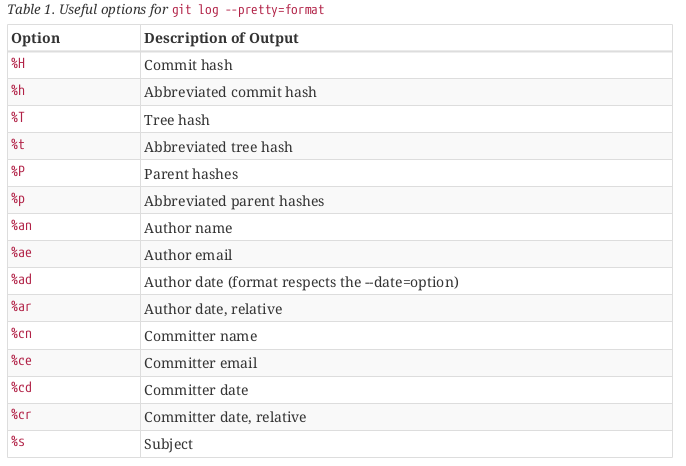
\includegraphics[scale=0.7]{./pic/tab_pretty.png}
\end{figure}

Finally we can also use :
\begin{lstlisting}
	<*\colorbox{gray!30!}{\textcolor{FireBrick}{git log --graph}}*>
	#Display will be like
	
	* commit cc012e3412018b9f6d8034ac93a4e65cbd355cba (git-svn)
	| Author: nsauraphd <nsauraphd@bef5c912-3013-4295-81d9-13fa92c63195>
	| Date:   Wed Oct 31 17:27:04 2018 +0000
	| 
	|     git-svn-id: https://subversion.renater.fr/mannt/trunk@437 	bef5c912-3013-4295-81d9-13fa92c63195
	| 
\end{lstlisting}

With the argument --since it is possible to limit the log outputs one can specify the threshold as :
\begin{itemize}
	\item[--] a date e.g.: "2008-01-15"; \\
	\item[--] or an amout of time "2 years 1 day 3 minutes ago" \\[4mm]
\end{itemize}

Another really helpful filter is the -S option, which takes a string and shows only those commits that changed the number of occurrences of that string. For instance, if you wanted to find the last commit that added or removed a reference to a specific function, you could call:
\begin{lstlisting}
	<*\colorbox{gray!30!}{\textcolor{FireBrick}{git log -S function\_name}}*>
\end{lstlisting}

\begin{figure}[!ht]
\centering
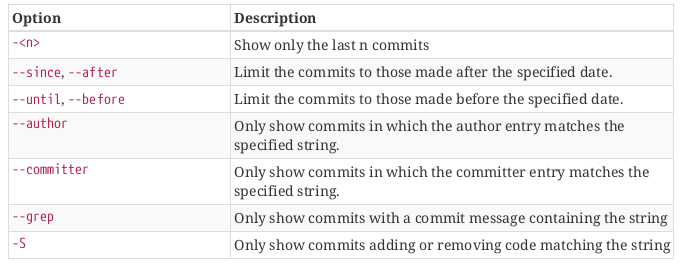
\includegraphics[scale=0.7]{./pic/tab_log.png}
\end{figure}

\pagebreak

\subsection*{Undoing things: how to undo}
The following will delete uncommitted changes :
\begin{lstlisting}
	<*\colorbox{gray!30!}{\textcolor{FireBrick}{git reset --hard HEAD}}*>
\end{lstlisting}

If we have just deleted a file, without commiting, for example : \textit{git rm bibli.txt}. We can cancel this deleting running :
\begin{lstlisting}
    <*\colorbox{gray!30!}{\textcolor{FireBrick}{git checkout HEAD ./bibli.txt}}*>
\end{lstlisting}

\textbf{Before the checkout} 
\begin{lstlisting}
saura@florian-OptiPlex-7010:~/Documents/Git_RANNS/ML$ git status
On branch master
Your branch is up to date with 'origin/master'.

Changes to be committed:
  (use "git reset HEAD <file>..." to unstage)

	deleted:    bibli.txt

\end{lstlisting}

\textbf{After the checkout :}

\begin{lstlisting}
saura@florian-OptiPlex-7010:~/Documents/Git_RANNS/ML$ git status
On branch master
Your branch is up to date with 'origin/master'.

nothing to commit, working tree clean

\end{lstlisting}

\pagebreak

\subsection*{The please tell me who you are error}
Happens when you want to modify a repositery without having initialized git.\\
This is the standard procedure to make a \textit{git push} works :
\begin{lstlisting}
	<*\colorbox{gray!30!}{\textcolor{FireBrick}{git init}}*>
	<*\colorbox{gray!30!}{\textcolor{FireBrick}{git config user.name «someone»}}*>
	<*\colorbox{gray!30!}{\textcolor{FireBrick}{git config user.email «somemail»}}*>
	<*\colorbox{gray!30!}{\textcolor{FireBrick}{git add $*$ }}*>
	<*\colorbox{gray!30!}{\textcolor{FireBrick}{git commit -m «somemessage»}}*>
\end{lstlisting}


\end{document}